\documentclass[12pt]{article}
\usepackage{amsthm,amssymb,amsfonts,amsmath,amstext,systeme}
\usepackage{graphicx,float}
\usepackage{tabularx}

\marginparwidth 0pt
\oddsidemargin -1.2 truecm
\evensidemargin  0pt 
\marginparsep 0pt
\topmargin -2.2truecm
\linespread{1}
\textheight 25.8 truecm
\textwidth 18.5 truecm
\newenvironment{remark}{\noindent{\bf Remark }}{\vspace{0mm}}
\newenvironment{remarks}{\noindent{\bf Remarks }}{\vspace{0mm}}
\newenvironment{question}{\noindent{\bf Question }}{\vspace{0mm}}
\newenvironment{questions}{\noindent{\bf Questions }}{\vspace{0mm}}
\newenvironment{note}{\noindent{\bf Note }}{\vspace{0mm}}
\newenvironment{summary}{\noindent{\bf Summary }}{\vspace{0mm}}
\newenvironment{back}{\noindent{\bf Background}}{\vspace{0mm}}
\newenvironment{conclude}{\noindent{\bf Conclusion}}{\vspace{0mm}}
\newenvironment{concludes}{\noindent{\bf Conclusions}}{\vspace{0mm}}
\newenvironment{dill}{\noindent{\bf Description of Dill's model}}{\vspace{0mm}}
\newenvironment{maths}{\noindent{\bf Mathematics needed}}{\vspace{0mm}}
\newenvironment{inst}{\noindent{\bf Instructions}}{\vspace{0mm}}
\newenvironment{notes}{\noindent{\bf Notes }}{\vspace{0mm}}
\newenvironment{theorem}{\noindent{\bf Theorem }}{\vspace{0mm}}
\newenvironment{example}{\noindent{\bf Example }}{\vspace{0mm}}
\newenvironment{examples}{\noindent{\bf Examples }}{\vspace{0mm}}
\newenvironment{topics}{\noindent{\bf Topics}}{\vspace{0mm}}
\newenvironment{outcomes}{\noindent{\bf Expected Learning Outcomes}}{\vspace{0mm}}
\newenvironment{lemma}{\noindent{\bf Lemma }}{\vspace{0mm}}
\newenvironment{solution}{\noindent{\it Solution}}{\vspace{2mm}}
\newcommand{\ds}{\displaystyle}
\newcommand{\un}{\underline}
\newcommand{\bs}{\boldsymbol}

\begin{document}

\baselineskip 18 pt
\begin{center}
	{\large \bf HKDSE MATH CORE 2022 Past Paper I}\\
	\vspace{2 mm}

\end{center}
\vspace{0.05cm}

\begin{enumerate}
	\item \textbf{HKDSE MATH CORE 2022 Past Paper I Q1}\\
	Simplify $\dfrac{(a^3b^{-2})^4}{a^{-5}b^6}$ and express your answer with positive indices. \\(3 marks)	
	
	\item \textbf{HKDSE MATH CORE 2022 Past Paper I Q2}\\
	Let $x$ and $y$ be two numbers. The sum of $x$ and $y$ is 456 while the product of 7 and $x$ is $y$. Find $x$. \\(3 marks)

	\item \textbf{HKDSE MATH CORE 2022 Past Paper I Q3}\\
	Simplify $\dfrac{3}{k - 9} + \dfrac{2}{5k + 6}$. \\(3 marks)

	\item \textbf{HKDSE MATH CORE 2022 Past Paper I Q4}\\
	Factorize
	\begin{enumerate}
		\item[(a)] $9c^2 - 6c + 1$,
		\item[(b)] $(4c + d)^2 - 9c^2 + 6c - 1$.
	\end{enumerate}
	(4 marks)

	\item \textbf{HKDSE MATH CORE 2022 Past Paper I Q5}\\
	A fan is sold at a discount of 30\% on its marked price. After selling the fan, the profit is \$78 and the percentage profit is 26\%. Find the marked price of the fan. \\(4 marks)

	\item \textbf{HKDSE MATH CORE 2022 Past Paper I Q6}\\
	Consider the compound inequality $$-2(3x + 2) > x + 10 \text{ or } 2x \leq -8 \dots\dots\dots\dots\dots (*) .$$
	\begin{enumerate}
		\item[(a)] Solve $(*)$.
		\item[(b)] Write down the greatest integer satisfying $(*)$.	
	\end{enumerate}
	(4 marks)

	\item \textbf{HKDSE MATH CORE 2022 Past Paper I Q7}\\
	The coordinates of the points $S$ and $T$ are $(12, -5)$ and $(-3, -7)$ respectively. $S$ is rotated anticlockwise about $O$ through $90^\circ$ to $S'$, where $O$ is the origin. $T'$ is the reflection image of $T$ with respect to the $x$-axis.
	\begin{enumerate}
		\item[(a)] Write down the coordinates of $S'$ and $T'$.
		\item[(b)] Find the slope of $S'T'$.
	\end{enumerate}
	(4 marks)
	
	\item \textbf{HKDSE MATH CORE 2022 Past Paper I Q8}\\
	In Figure 1, $A$ is a poinjt lying inside the quadrilateral $BCDE$ such that $AC // ED$ and $AD // BC$. It is given that $\angle ABD = \angle AED$ and $AB = AE$.
	\begin{figure}[H]
		\centering
		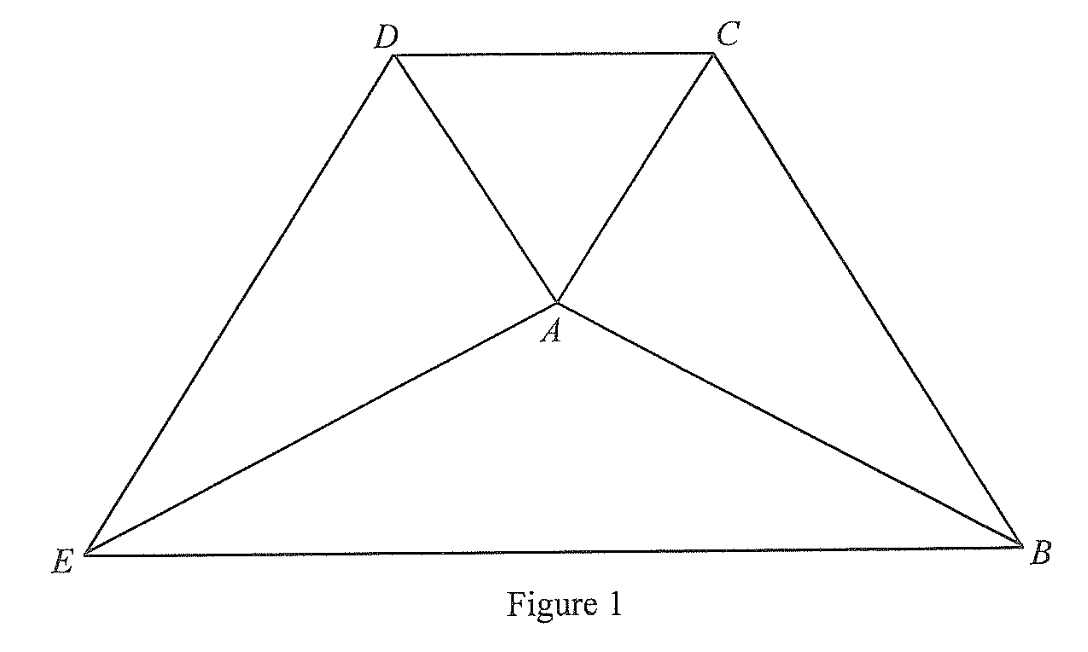
\includegraphics[width = .3\linewidth]{2022Figure1.1}
	\end{figure}
	\begin{enumerate}
		\item[(a)] Prove that $\triangle ABC \cong \triangle AED$.
		\item[(b)] If $\angle ABC = 39^\circ$ and $\angle DAE = 87^\circ$, find $\angle ACD$.
	\end{enumerate}
	(5 marks)	
	
	\item \textbf{HKDSE MATH CORE 2022 Past Paper I Q9}\\
	The frequency distribution table and the cumulative frequency distribution table below show the distribution of the times taken to complete a 3 km race by a group of students.
	\begin{table}[h]
		\centering
		\begin{minipage}{.4\textwidth}
		  \centering
		  \begin{tabular}{ | c | c | }
			\hline
			Time taken (minutes) & Frequency \\
			\hline
			$10 - 14$ & $a$ \\
			\hline			
			$15 - 19$ & 9 \\
			\hline
			$20 - 24$ & $b$ \\
			\hline
			$25 - 29$ & 3 \\
			\hline
		  \end{tabular}
		\end{minipage}
		%\hfill
		\begin{minipage}{.5\textwidth}
		  \centering
		  \begin{tabular}{ | c | c | }
			\hline
			Time taken less than(minutes) & Cumulative frequency\\
			\hline
			14.5 & 3 \\
			\hline
			19.5 & $x$ \\
			\hline
			24.5 & $y$ \\
			\hline
			29.5 & 20 \\
			\hline
		  \end{tabular}
		\end{minipage}
		\label{tab:two_tables}
	\end{table}
	\begin{enumerate}
		\item[(a)] Write down the value of $x$.
		\item[(b)] Find the mean of the distribution.
		\item[(c)] Find the probability that the time taken to complete the 3 km race by a randomly selected student from the group is less than 19.5 minutes.
	\end{enumerate}
	(5 marks)

	\item \textbf{HKDSE MATH CORE 2022 Past Paper I Q10}\\
	It is given that $f(x)$ partly varies as $x^2$ and partly varies as $x$. Suppose that $f(4) = 96$ and $f(-5) = 15$.
	\begin{enumerate}
		\item[(a)] Find $f(x)$. \\(3 marks)
		\item[(b)] Wrtie down the $x$-intercept of the graph of $y = 8f(x)$. \\(1 marks)
		\item[(c)] Let $k$ be a real constant. Find the range of values of $k$ such that the equation $f(x) = k$ has two distinct real roots. \\(2 marks)
	\end{enumerate}

	\item \textbf{HKDSE MATH CORE 2022 Past Paper I Q11}\\
	The stem-and-leaf diagram below shows the distribution of the ages of the players of a football team.
	\begin{table}[htbp]
		\centering
		\begin{tabular}{r|l@{\hspace{4 pt}}l@{\hspace{4 pt}}l@{\hspace{4 pt}}l@{\hspace{4 pt}}}
		   Stem (tens) & Leaf (units)     \\
			\hline
			1     & 7 8 9\\    
			2     & 0 $a$ $a$ 8 8 9\\    
			3     & $b$ $b$ 5 5 6 6 6 6 7 8\\    
			4     & 3\\
		\end{tabular}
	\end{table}
	The inter-quartile range and the median of the distribution are 14 and 31 respectively.
	\begin{enumerate}
		\item[(a)] Find $a$ and $b$. \\(3 marks)
		\item[(b)] A player now leaves the football team.
		\begin{enumerate}
			\item[(i)] Is there any change in the mode of the distribution due to the leaving of the player? Explain your answer.
			\item[(ii)] If the range of the distribution is decreased, find the greatest possible standard deviation of the distribution.
		\end{enumerate}
		(4 marks)
	\end{enumerate}

	\item \textbf{HKDSE MATH CORE 2022 Past Paper I Q12}\\
	The equation of the circle $C$ is $x^2 + y^2 - 154x - 128y + 224 = 0$. Denote the centre of $C$ by $G$. The coordinates of the point $H$ are $(65, 48)$.
	\begin{enumerate}
		\item[(a)] Find the distance between $G$ and $H$. \\(3 marks)
		\item[(b)] Let $P$ be a moving point on $C$. When the area of $\triangle GHP$ is the greatest,
		\begin{enumerate}
			\item[(i)] describe the geometric relationship between $GH$ and $GP$;
			\item[(ii)] find the perimeter of $\triangle GHP$.
		\end{enumerate}
		(4 marks)
	\end{enumerate}

	\item \textbf{HKDSE MATH CORE 2022 Past Paper I Q13}\\
	There are two solid metal spheres. The ration of the surface area of the smaller sphere to the surface area of the larger sphere is 4:9. The radius of the larger sphere 9 cm.
	\begin{enumerate}
		\item[(a)] Express, in terms of $\pi$, the volume of the smaller sphere. \\(3 marks)
		\item[(b)] The two spheres are melted and recast into two solid right circular cones. Denote these two circular cones by $A$ and $B$. It is given tha tht eheight and the base radius $A$ are 10 cm and 6 cm respectively. A student finds thatthe base radius of $B$ is 12 cm. The student claims that $A$ and $B$ are similar. Is the claim correct? Explain your answer. \\(4 marks)
	\end{enumerate}

	\item \textbf{HKDSE MATH CORE 2022 Past Paper I Q14}\\
	Let $p(x) = 2x^3 + ax^2 + bx - 20$, where $a$ and $b$ are constants. When $p(x)$ is divided by $x^2 - 2x + 3$, the remainder is $x + 13$.
	\begin{enumerate}
		\item[(a)] Find $a$ and $b$. \\(3 marks)
		\item[(b)] Is $x - 5$ a factor of $p(x)$? Explain your answer. \\(2 marks)
		\item[(c)] Someone claims that the equation $p(x) = 0$ has two irrational roots. Do you agree? Explain your answer. \\(3 marks)
	\end{enumerate}

	\item \textbf{HKDSE MATH CORE 2022 Past Paper I Q15}\\
	There are 10 boys and 12 girls in a class. If 4 students are randomly selected from the class to form a committee.
	\begin{enumerate}
		\item[(a)] find the probability that there are 2 boys and 2 girls in the committee. \\(2 marks)
		\item[(b)] find the probability that the number of boys and the number of girls in the committee are different. \\(2 marks)
	\end{enumerate}

	\item \textbf{HKDSE MATH CORE 2022 Past Paper I Q16}\\
	Let $g(x) = 3x^2 + 12kx^2 + 16k^2 + 8$, where $k$ is a non-zero constant.
	\begin{enumerate}
		\item[(a)] Using the method of completing the square, express, in terms of $k$, the coordinates of the vertex of the graph of $y = g(x)$. \\(2 marks) 
		\item[(b)] On the same rectangular coordinates system, denote the vertex of the graph of $y = g(x)$ and the vertex of the graph of $y = 2g(-x)$ by $A$ and $B$ respectively. Let $M$ be a point lying on $AB$ such that the area of $\triangle OBM$ is the triple of the area of $\triangle OAM$, where $O$ is the origin. Express, in terms of $k$, the coordinates of $M$. \\(3 marks)
	\end{enumerate}

	\item \textbf{HKDSE MATH CORE 2022 Past Paper I Q17}\\
	Let $c$ be a real constant. The roots of the equation $x^2 + cx - 9 = 0$ are $\alpha$ and $\beta$.
	\begin{enumerate}
		\item[(a)] Express $\alpha^2 + \beta^2$ in terms of $c$. \\(3 marks)
		\item[(b)] The 1st term, the 2nd term and the 3rd term of an arithmetic sequence are $c^2$, $\alpha^2 + \beta^2$ and 85 respectively. Find the least value of $n$ such that the sum of the first $n$ terms of the sequence is greater than $2 \times 10^6$. \\(4 marks)
	\end{enumerate}

	\item \textbf{HKDSE MATH CORE 2022 Past Paper I Q18}\\
	In Figure 2, the triangular paper and $PQR$ is held such that $PQ$ lies on the horizontal ground. It is given that $PQ = 30$ cm, $PR = 25$ cm and $\angle QPR = 95
	^\circ$.
	\begin{figure}[H]
		\centering
		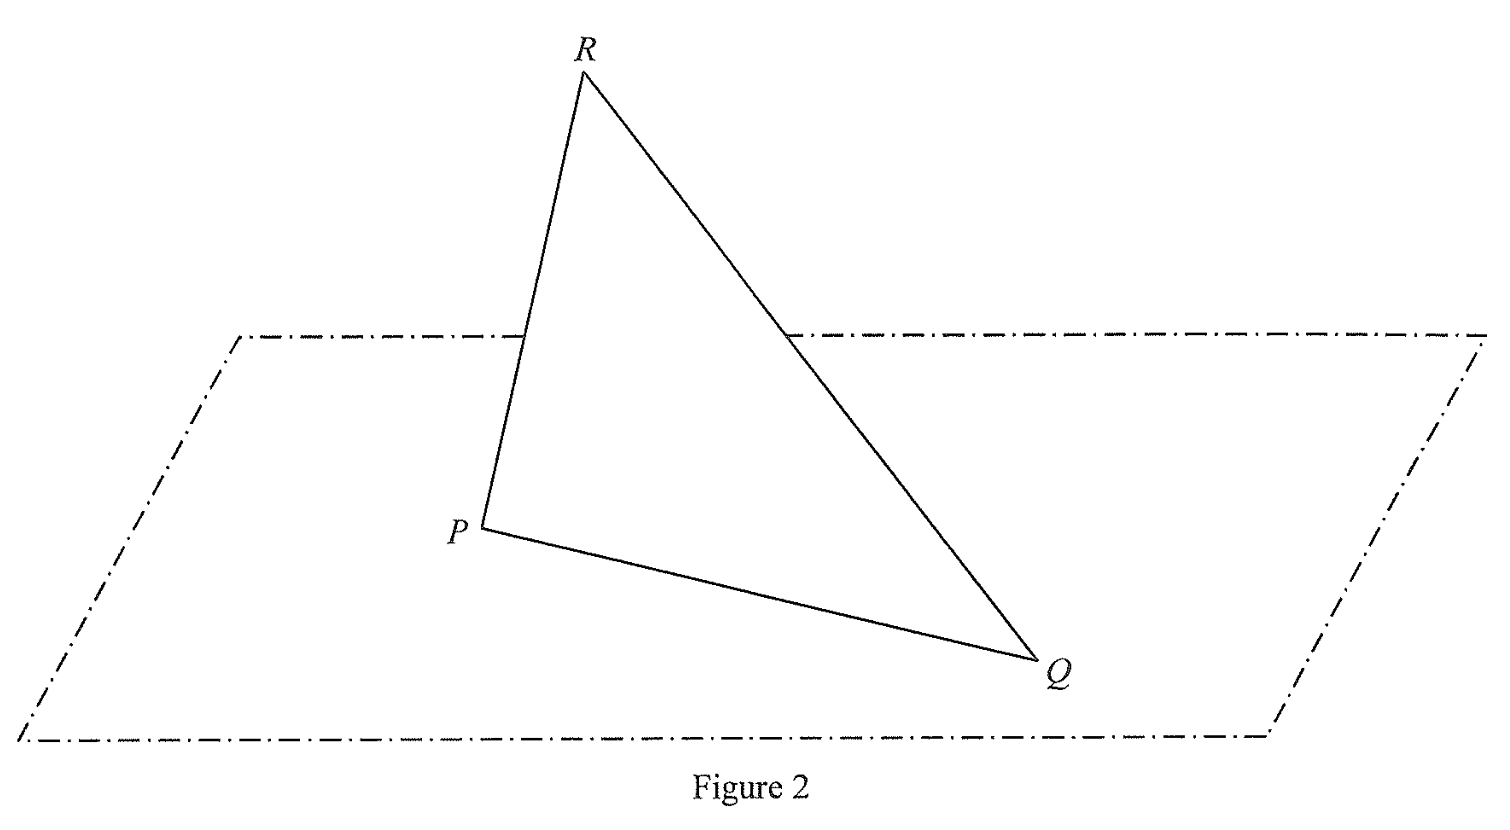
\includegraphics[width = .3\linewidth]{2022Figure1.2}
	\end{figure}
	\begin{enumerate}
		\item[(a)] Find
		\begin{enumerate}
			\item[(i)] the length of $QR$,
			\item[(ii)] $\angle PQR$.
		\end{enumerate}
		(4 marks)
		\item[(b)] Let $M$ be the mid-point of $QR$. A craftman finds that the angle between $PR$ and the horizontal ground is $70^\circ$. The craftman claims that the angle between $PM$ and the horizontal ground exceeds $40^\circ$. Is the claim correct? Explain your answer. \\(3 marks)
	\end{enumerate}

	\item \textbf{HKDSE MATH CORE 2022 Past Paper I Q19}\\
	The centre of the circle $C$ is the point $G(83, 112)$. It is found that the point $A(158, 12)$ lies outside $C$, $AP$ and $AQ$ are the tangents to $C$ at the points $P$ and $Q$ respectively. It is given that $C$ passes through the point $(23, 67)$.
	\begin{enumerate}
		\item[(a)] Find the equation of the straight line passing through $A$ and $G$. \\(2 marks)
		\item[(b)] Find the coordinates of the point of intersection of $AG$ and $PQ$. \\(3 marks)
		\item[(c)] Find the equation of the inscribed circle of $\triangle APQ$. \\(4 marks)
		\item[(d)] Someone claims that the ratio of the area of the inscribed circle to the area of the circumcircle of $\triangle APQ$ is 1 : 4. Do you agree? Explain your answer. \\(3 marks)
	\end{enumerate}


\end{enumerate}
\end{document}